
%% bare_conf.tex
%% V1.4b
%% 2015/08/26
%% by Michael Shell
%% See:
%% http://www.michaelshell.org/
%% for current contact information.
%%
%% This is a skeleton file demonstrating the use of IEEEtran.cls
%% (requires IEEEtran.cls version 1.8b or later) with an IEEE
%% conference paper.
%%
%% Support sites:
%% http://www.michaelshell.org/tex/ieeetran/
%% http://www.ctan.org/pkg/ieeetran
%% and
%% http://www.ieee.org/

%%*************************************************************************
%% Legal Notice:
%% This code is offered as-is without any warranty either expressed or
%% implied; without even the implied warranty of MERCHANTABILITY or
%% FITNESS FOR A PARTICULAR PURPOSE! 
%% User assumes all risk.
%% In no event shall the IEEE or any contributor to this code be liable for
%% any damages or losses, including, but not limited to, incidental,
%% consequential, or any other damages, resulting from the use or misuse
%% of any information contained here.
%%
%% All comments are the opinions of their respective authors and are not
%% necessarily endorsed by the IEEE.
%%
%% This work is distributed under the LaTeX Project Public License (LPPL)
%% ( http://www.latex-project.org/ ) version 1.3, and may be freely used,
%% distributed and modified. A copy of the LPPL, version 1.3, is included
%% in the base LaTeX documentation of all distributions of LaTeX released
%% 2003/12/01 or later.
%% Retain all contribution notices and credits.
%% ** Modified files should be clearly indicated as such, including  **
%% ** renaming them and changing author support contact information. **
%%*************************************************************************


% *** Authors should verify (and, if needed, correct) their LaTeX system  ***
% *** with the testflow diagnostic prior to trusting their LaTeX platform ***
% *** with production work. The IEEE's font choices and paper sizes can   ***
% *** trigger bugs that do not appear when using other class files.       ***                          ***
% The testflow support page is at:
% http://www.michaelshell.org/tex/testflow/



\documentclass[conference]{IEEEtran}
\usepackage[utf8]{inputenc}
% Some Computer Society conferences also require the compsoc mode option,
% but others use the standard conference format.
%
% If IEEEtran.cls has not been installed into the LaTeX system files,
% manually specify the path to it like:
% \documentclass[conference]{../sty/IEEEtran}


\usepackage[draft,danish]{fixme}


% Some very useful LaTeX packages include:
% (uncomment the ones you want to load)


% *** MISC UTILITY PACKAGES ***
%
%\usepackage{ifpdf}
% Heiko Oberdiek's ifpdf.sty is very useful if you need conditional
% compilation based on whether the output is pdf or dvi.
% usage:
% \ifpdf
%   % pdf code
% \else
%   % dvi code
% \fi
% The latest version of ifpdf.sty can be obtained from:
% http://www.ctan.org/pkg/ifpdf
% Also, note that IEEEtran.cls V1.7 and later provides a builtin
% \ifCLASSINFOpdf conditional that works the same way.
% When switching from latex to pdflatex and vice-versa, the compiler may
% have to be run twice to clear warning/error messages.






% *** CITATION PACKAGES ***
%
\usepackage{cite}
% cite.sty was written by Donald Arseneau
% V1.6 and later of IEEEtran pre-defines the format of the cite.sty package
% \cite{} output to follow that of the IEEE. Loading the cite package will
% result in citation numbers being automatically sorted and properly
% "compressed/ranged". e.g., [1], [9], [2], [7], [5], [6] without using
% cite.sty will become [1], [2], [5]--[7], [9] using cite.sty. cite.sty's
% \cite will automatically add leading space, if needed. Use cite.sty's
% noadjust option (cite.sty V3.8 and later) if you want to turn this off
% such as if a citation ever needs to be enclosed in parenthesis.
% cite.sty is already installed on most LaTeX systems. Be sure and use
% version 5.0 (2009-03-20) and later if using hyperref.sty.
% The latest version can be obtained at:
% http://www.ctan.org/pkg/cite
% The documentation is contained in the cite.sty file itself.






% *** GRAPHICS RELATED PACKAGES ***
%
\ifCLASSINFOpdf
   \usepackage[pdftex]{graphicx}
  % declare the path(s) where your graphic files are
  % \graphicspath{{../pdf/}{../jpeg/}}
  \graphicspath{{figures/}}
  % and their extensions so you won't have to specify these with
  % every instance of \includegraphics
  % \DeclareGraphicsExtensions{.pdf,.jpeg,.png}
\else
  % or other class option (dvipsone, dvipdf, if not using dvips). graphicx
  % will default to the driver specified in the system graphics.cfg if no
  % driver is specified.
  % \usepackage[dvips]{graphicx}
  % declare the path(s) where your graphic files are
  % \graphicspath{{../eps/}}
  % and their extensions so you won't have to specify these with
  % every instance of \includegraphics
  % \DeclareGraphicsExtensions{.eps}
\fi
% graphicx was written by David Carlisle and Sebastian Rahtz. It is
% required if you want graphics, photos, etc. graphicx.sty is already
% installed on most LaTeX systems. The latest version and documentation
% can be obtained at: 
% http://www.ctan.org/pkg/graphicx
% Another good source of documentation is "Using Imported Graphics in
% LaTeX2e" by Keith Reckdahl which can be found at:
% http://www.ctan.org/pkg/epslatex
%
% latex, and pdflatex in dvi mode, support graphics in encapsulated
% postscript (.eps) format. pdflatex in pdf mode supports graphics
% in .pdf, .jpeg, .png and .mps (metapost) formats. Users should ensure
% that all non-photo figures use a vector format (.eps, .pdf, .mps) and
% not a bitmapped formats (.jpeg, .png). The IEEE frowns on bitmapped formats
% which can result in "jaggedy"/blurry rendering of lines and letters as
% well as large increases in file sizes.
%
% You can find documentation about the pdfTeX application at:
% http://www.tug.org/applications/pdftex





% *** MATH PACKAGES ***
%
\usepackage{amsmath}

% A popular package from the American Mathematical Society that provides
% many useful and powerful commands for dealing with mathematics.
%
% Note that the amsmath package sets \interdisplaylinepenalty to 10000
% thus preventing page breaks from occurring within multiline equations. Use:
\interdisplaylinepenalty=2500
% after loading amsmath to restore such page breaks as IEEEtran.cls normally
% does. amsmath.sty is already installed on most LaTeX systems. The latest
% version and documentation can be obtained at:
% http://www.ctan.org/pkg/amsmath





% *** SPECIALIZED LIST PACKAGES ***
%
%\usepackage{algorithmic}
% algorithmic.sty was written by Peter Williams and Rogerio Brito.
% This package provides an algorithmic environment fo describing algorithms.
% You can use the algorithmic environment in-text or within a figure
% environment to provide for a floating algorithm. Do NOT use the algorithm
% floating environment provided by algorithm.sty (by the same authors) or
% algorithm2e.sty (by Christophe Fiorio) as the IEEE does not use dedicated
% algorithm float types and packages that provide these will not provide
% correct IEEE style captions. The latest version and documentation of
% algorithmic.sty can be obtained at:
% http://www.ctan.org/pkg/algorithms
% Also of interest may be the (relatively newer and more customizable)
% algorithmicx.sty package by Szasz Janos:
% http://www.ctan.org/pkg/algorithmicx




% *** ALIGNMENT PACKAGES ***
%
\usepackage{array}
% Frank Mittelbach's and David Carlisle's array.sty patches and improves
% the standard LaTeX2e array and tabular environments to provide better
% appearance and additional user controls. As the default LaTeX2e table
% generation code is lacking to the point of almost being broken with
% respect to the quality of the end results, all users are strongly
% advised to use an enhanced (at the very least that provided by array.sty)
% set of table tools. array.sty is already installed on most systems. The
% latest version and documentation can be obtained at:
% http://www.ctan.org/pkg/array


% IEEEtran contains the IEEEeqnarray family of commands that can be used to
% generate multiline equations as well as matrices, tables, etc., of high
% quality.




% *** SUBFIGURE PACKAGES ***
%\ifCLASSOPTIONcompsoc
%  \usepackage[caption=false,font=normalsize,labelfont=sf,textfont=sf]{subfig}
%\else
%  \usepackage[caption=false,font=footnotesize]{subfig}
%\fi
% subfig.sty, written by Steven Douglas Cochran, is the modern replacement
% for subfigure.sty, the latter of which is no longer maintained and is
% incompatible with some LaTeX packages including fixltx2e. However,
% subfig.sty requires and automatically loads Axel Sommerfeldt's caption.sty
% which will override IEEEtran.cls' handling of captions and this will result
% in non-IEEE style figure/table captions. To prevent this problem, be sure
% and invoke subfig.sty's "caption=false" package option (available since
% subfig.sty version 1.3, 2005/06/28) as this is will preserve IEEEtran.cls
% handling of captions.
% Note that the Computer Society format requires a larger sans serif font
% than the serif footnote size font used in traditional IEEE formatting
% and thus the need to invoke different subfig.sty package options depending
% on whether compsoc mode has been enabled.
%
% The latest version and documentation of subfig.sty can be obtained at:
% http://www.ctan.org/pkg/subfig




% *** FLOAT PACKAGES ***
%
%\usepackage{fixltx2e}
% fixltx2e, the successor to the earlier fix2col.sty, was written by
% Frank Mittelbach and David Carlisle. This package corrects a few problems
% in the LaTeX2e kernel, the most notable of which is that in current
% LaTeX2e releases, the ordering of single and double column floats is not
% guaranteed to be preserved. Thus, an unpatched LaTeX2e can allow a
% single column figure to be placed prior to an earlier double column
% figure.
% Be aware that LaTeX2e kernels dated 2015 and later have fixltx2e.sty's
% corrections already built into the system in which case a warning will
% be issued if an attempt is made to load fixltx2e.sty as it is no longer
% needed.
% The latest version and documentation can be found at:
% http://www.ctan.org/pkg/fixltx2e


\usepackage{stfloats}
% stfloats.sty was written by Sigitas Tolusis. This package gives LaTeX2e
% the ability to do double column floats at the bottom of the page as well
% as the top. (e.g., "\begin{figure*}[!b]" is not normally possible in
% LaTeX2e). It also provides a command:
%\fnbelowfloat
% to enable the placement of footnotes below bottom floats (the standard
% LaTeX2e kernel puts them above bottom floats). This is an invasive package
% which rewrites many portions of the LaTeX2e float routines. It may not work
% with other packages that modify the LaTeX2e float routines. The latest
% version and documentation can be obtained at:
% http://www.ctan.org/pkg/stfloats
% Do not use the stfloats baselinefloat ability as the IEEE does not allow
% \baselineskip to stretch. Authors submitting work to the IEEE should note
% that the IEEE rarely uses double column equations and that authors should try
% to avoid such use. Do not be tempted to use the cuted.sty or midfloat.sty
% packages (also by Sigitas Tolusis) as the IEEE does not format its papers in
% such ways.
% Do not attempt to use stfloats with fixltx2e as they are incompatible.
% Instead, use Morten Hogholm'a dblfloatfix which combines the features
% of both fixltx2e and stfloats:
%
% \usepackage{dblfloatfix}
% The latest version can be found at:
% http://www.ctan.org/pkg/dblfloatfix

\usepackage{hyperref}
\hypersetup{%
	%pdfpagelabels=true,%
	plainpages=false,%
	pdfauthor={Author(s)},%
	pdftitle={Title},%
	pdfsubject={Subject},%
	bookmarksnumbered=true,%
	colorlinks,%
	citecolor=black,%
	filecolor=black,%
	linkcolor=black,% you should probably change this to black before printing
	urlcolor=black,%
	pdfstartview=FitH%
}
\renewcommand*{\figureautorefname}{Fig.}

% *** PDF, URL AND HYPERLINK PACKAGES ***
%
\usepackage{url}
% url.sty was written by Donald Arseneau. It provides better support for
% handling and breaking URLs. url.sty is already installed on most LaTeX
% systems. The latest version and documentation can be obtained at:
% http://www.ctan.org/pkg/url
% Basically, \url{my_url_here}.




% *** Do not adjust lengths that control margins, column widths, etc. ***
% *** Do not use packages that alter fonts (such as pslatex).         ***
% There should be no need to do such things with IEEEtran.cls V1.6 and later.
% (Unless specifically asked to do so by the journal or conference you plan
% to submit to, of course. )


% correct bad hyphenation here
\hyphenation{op-tical net-works semi-conduc-tor}
\bibliographystyle{setup/IEEEtran}

\begin{document}
%
% paper title
% Titles are generally capitalized except for words such as a, an, and, as,
% at, but, by, for, in, nor, of, on, or, the, to and up, which are usually
% not capitalized unless they are the first or last word of the title.
% Linebreaks \\ can be used within to get better formatting as desired.
% Do not put math or special symbols in the title.
\title{Validation of Path Loss for \\ Near-Ground Sensor Networks}


% author names and affiliations
% use a multiple column layout for up to three different
% affiliations
\author{\IEEEauthorblockN{Thomas Jørgensen}
\IEEEauthorblockA{7. semester, Wireless\\\ Communication Systems \\
 Aalborg University\\
Email: tkjj13@student.aau.dk}
\and
\IEEEauthorblockN{Kemal Kapetanovic}
\IEEEauthorblockA{7. semester, Wireless\\\ Communication Systems \\
Aalborg University\\
Email: kkapet08@student.aau.dk}
\and
\IEEEauthorblockN{Mads Gotthardsen}
\IEEEauthorblockA{7. semester, Wireless\\\ Communication Systems \\
Aalborg University\\
Email: mgotth13@student.aau.dk}}

% conference papers do not typically use \thanks and this command
% is locked out in conference mode. If really needed, such as for
% the acknowledgment of grants, issue a \IEEEoverridecommandlockouts
% after \documentclass

% for over three affiliations, or if they all won't fit within the width
% of the page, use this alternative format:
% 
%\author{\IEEEauthorblockN{Michael Shell\IEEEauthorrefmark{1},
%Homer Simpson\IEEEauthorrefmark{2},
%James Kirk\IEEEauthorrefmark{3}, 
%Montgomery Scott\IEEEauthorrefmark{3} and
%Eldon Tyrell\IEEEauthorrefmark{4}}
%\IEEEauthorblockA{\IEEEauthorrefmark{1}School of Electrical and Computer Engineering\\
%Georgia Institute of Technology,
%Atlanta, Georgia 30332--0250\\ Email: see http://www.michaelshell.org/contact.html}
%\IEEEauthorblockA{\IEEEauthorrefmark{2}Twentieth Century Fox, Springfield, USA\\
%Email: homer@thesimpsons.com}
%\IEEEauthorblockA{\IEEEauthorrefmark{3}Starfleet Academy, San Francisco, California 96678-2391\\
%Telephone: (800) 555--1212, Fax: (888) 555--1212}
%\IEEEauthorblockA{\IEEEauthorrefmark{4}Tyrell Inc., 123 Replicant Street, Los Angeles, California 90210--4321}}




% use for special paper notices
%\IEEEspecialpapernotice{(Invited Paper)}




% make the title area
\maketitle

% As a general rule, do not put math, special symbols or citations
% in the abstract
\begin{abstract}
The abstract goes here.
\end{abstract}

% no keywords




% For peer review papers, you can put extra information on the cover
% page as needed:
% \ifCLASSOPTIONpeerreview
% \begin{center} \bfseries EDICS Category: 3-BBND \end{center}
% \fi
%
% For peerreview papers, this IEEEtran command inserts a page break and
% creates the second title. It will be ignored for other modes.
\IEEEpeerreviewmaketitle



\section{Introduction}

In the future it is likely that more and more wireless sensor networks (WSN) will appear. Many of such networks may be placed close to or directly in the ground for instance to monitor traffic flow or home power consumption examples could also include industrial or military uses. In such networks both power efficiency as well as reliability is key. To estimates those a reliable model for the path loss (PL) is needed. When placing the antenna so close to the ground a few problems occur, these problems still needs to be investigated further to effectively estimate the PL. Many of the earliest works only focus on frequencies below 30 MHz \cite{Bullington}, and states that the complexity increases as frequency increases. 


%The problem about calculating the path loss for antennas located near ground has been looked on.

\subsection{Path loss models}

In terms of calculating the PL, different propagation models can be applied, to calculate the power received, given different conditions. One of the more extensive models is the Ground Wave Path Loss (GWPL) model. The GWPL model takes the three most dominant factors into account when calculating the PL \cite{Chong,Bullington}, the direct wave the reflected wave and the surface wave.  


\begin{equation}
P_r=P_0 \cdot \Big|\underbrace{1}_{\begin{subarray}{c}Direct\\wave\end{subarray}}+\underbrace{R\text{e}^{j\Delta}}_{\begin{subarray}{c}Reflected\\wave\end{subarray}}+\underbrace{(1-R)A\text{e}^{j\Delta}}_{\begin{subarray}{c}Surface\\wave\end{subarray}}\Big|^2 
\label{ground_wave}
\end{equation}
where
\begin{equation}
P_0 = \frac{P_t G_t G_r}{L} \left(\frac{\lambda}{4 \pi d}\right)^2 
\label{ground_wave_P0}
\end{equation}

$P_{r}$ and $P_{t}$ are the power received and transmitted respectively, $G_t$ and $G_r$ are the gains in the transmitting and receiving antenna respectively, $L$ is the system loss, $\lambda$ is the wavelength of the transmitted signal, $d$ is the distance between the transmitting and receiving antenna, $\Delta$ is the phase difference between the direct and reflected wave, $R$ is the complex reflection coefficient and $A$ is the surface wave attenuation factor \cite{Chong,Bullington}. 

%$\Delta$ $\approx$ $\frac{4\pi h_{r} h_{t}}{\lambda d}$

The complex reflection coefficient \eqref{reflection_coefficient} is dependent on the incidence angle and the surface materiel.
\begin{equation}
R = \frac{\sin(\theta)-z}{\sin(\theta)-z}
\label{reflection_coefficient}
\end{equation}

where $\theta$ is the incidence angle, and where $z$ is different for vertical or horizontal polarization, and respectively given as.

\begin{align}
z &= \frac{\sqrt{\epsilon_{0}-\cos^{2}\theta}}{\epsilon_{0}} \\
z &= \sqrt{\epsilon_{0}-\cos^{2}\theta}
\end{align}

where $\epsilon_{0}$ is the Complex relative permittivity for the surface and can be found using the methods described in \cite{Kim}.\\
The surface wave attenuation factor can approximated as \eqref{attenuation_factor_A}\cite{Chong, Bullington}. 


\begin{equation}
A \approx \frac{-1}{1+j\frac{2\pi d}{\lambda}(\sin(\theta)+z)^{2}}
\label{attenuation_factor_A}
\end{equation}


As the GWPL model is quite complex different approximations of it has been made that makes it possible to calculate the PL without making measurements of the environment. The most simple model is the Friss free space path loss (FSPL) model \eqref{simple_friss} which calculates the power received, given only free space loss \cite{Chong}. This means that the reflected wave and surface wave can be set to 0 in \eqref{ground_wave}. 

\begin{equation}
P_r = \frac{P_t G_t G_r}{L} \left(\frac{\lambda}{4 \pi d}\right)^2
\label{simple_friss}
\end{equation}

This model \eqref{simple_friss} is not the the complete FSPL, as it assumes no losses due to polarization mismatch, pointing error, and matching between the system and antennas \cite{full_friss}. \\



As the FSPL only accounts for the direct wave between the receiver and the transmitter. A model that also accounts for the single point reflected wave is the two-ray-ground-reflection path loss model (TRPL) \eqref{two_ray_model} \cite{two_ray}. 

\begin{equation}
P_r(d) = \frac{P_t G_t G_r }{L}\left(\frac{h_t h_r}{d^2}\right)^2
\label{two_ray_model}
\end{equation}

where $h_t$, $h_r$ are the heights of the transmitting and receiving antenna respectively. \\
From the complete ground wave model given in \eqref{ground_wave}, the TRLP can be simplified to \eqref{two_ray_model}, when $\frac{\Delta}{2}$ $<$ $\pi$/$10$ $\Rightarrow$ $\sin$ $\frac{\Delta}{2}$ $\approx$ $\frac{\Delta}{2}$. This approximation holds when \eqref{two_ray_cond} is true and thus the simplified TRPL \eqref{two_ray_model} can be applied. If \eqref{two_ray_cond} is false FSPL \eqref{simple_friss} can be applied.
  
\begin{equation}
d > \frac{4\pi \cdot h_t h_r }{\lambda}
\label{two_ray_cond}
\end{equation}
 

The condition \eqref{two_ray_cond}, exists because the TRPL model considers two waves, a direct and a reflected wave, which interferes in an alternating constructive or destructive manner.

%\begin{equation}
%P_r(d) = \frac{P_t G_t G_r }{L}\left(\frac{h_t h_r}{d^2}\right)^2
%\label{two_ray_model}
%\end{equation}

%where $h_t$, $h_r$ are the heights of the transmitting and receiving antenna respectively. \\
%As the TRPL model considers two waves, a direct and a reflected wave, this model predicts interferences, which are caused by the constructive and destructive combination of the two waves. The interference is dominant if \eqref{two_ray_cond} is true\cite{two_ray}.


%this gives the following condition:


%a condition is introduced given as:

%\begin{equation}
%d < d_{c}
%\label{two_ray_cond}
%\end{equation}

%where %$d_{c}$ is called the cross over distance and is given as:

%\begin{equation}
%d_{c} = \frac{4\pi \cdot h^2_t h^2_r }{\lambda}
%\label{two_ray_cross_dis}
%\end{equation}  

However when placing the antennas at ground level, the TRLP predicts that the power received is zero, which is not the case.
The reason is that the surface wave becomes relevant \cite{Chong}. The surface wave assumes a minimum effective height of the antennas as can be seen in \eqref{surface_wave}. 

\begin{equation}
P_r=\frac{P_t G_t G_r }{L}\left(\frac{h_0}{d}\right)^4
\label{surface_wave}
\end{equation}

where $h_0$ is the minimum effective height of the antennas. 

\begin{equation}
h_{0} = \left|\frac{\lambda}{2\pi z}\right|
\label{h_0}
\end{equation}

This equation assume that $\Delta \approx 0$ and the reflection coefficient $\approx -1$ in the GWPL model \cite{Chong}. The condition in terms of when to use the surface wave \eqref{surface_wave} is dependent on the height of the antennas \cite{Chong}.
\begin{equation}
h_{r,t} < \lambda
\label{cond_surface}
\end{equation}
When \eqref{cond_surface} is true the FSPL and TRPL respectively under and overestimate the PL.

\subsection{Method}
To solve a problem like this there is generally two types of approaches a theoretic approach where the models are derieved using physics and electromagnetism and an experimental approach where the PL is measured and a model is fitted to the data. This article will focus on validation of existing models using experiments. 

The validation will be made over multiple steps, the first is to assume no knowledge of existing model and design a measurement campaign which accounts for all possible parameters that might affect the PL. The next step is to try and exclude parameters that have little to no statistical influence on the PL. Lastly the data will be matched with the data to verify if the model predicts the PL within an acceptable margin.  

\section{Methods and materials}
A experiential method based on measurements is used to make the PL model, that will be used to calculate the loss for near ground communication. This model is based on data gathered from measuring the PL at different heights and distances. In each point there will be taken multiple measurements, so the noise factor will have a less of an effect on the results.

During testing, five sets of antennas are used, a set monopole antennas (858 MHz) a set patch antennas (858 MHz). By using two different sets of antennas, it can be taken into account if the antenna type will have a influence on the results of the measurements. 

There will also be tested with horizontal and vertical polarization, to see if this will effect the model. The testing will take place at two locations, outside an empty parking lot and inside a gym (45 by 25 meters). Two locations is used, to see if the model works at two different locations.

%\begin{figure}[!htbp]
%\centering
%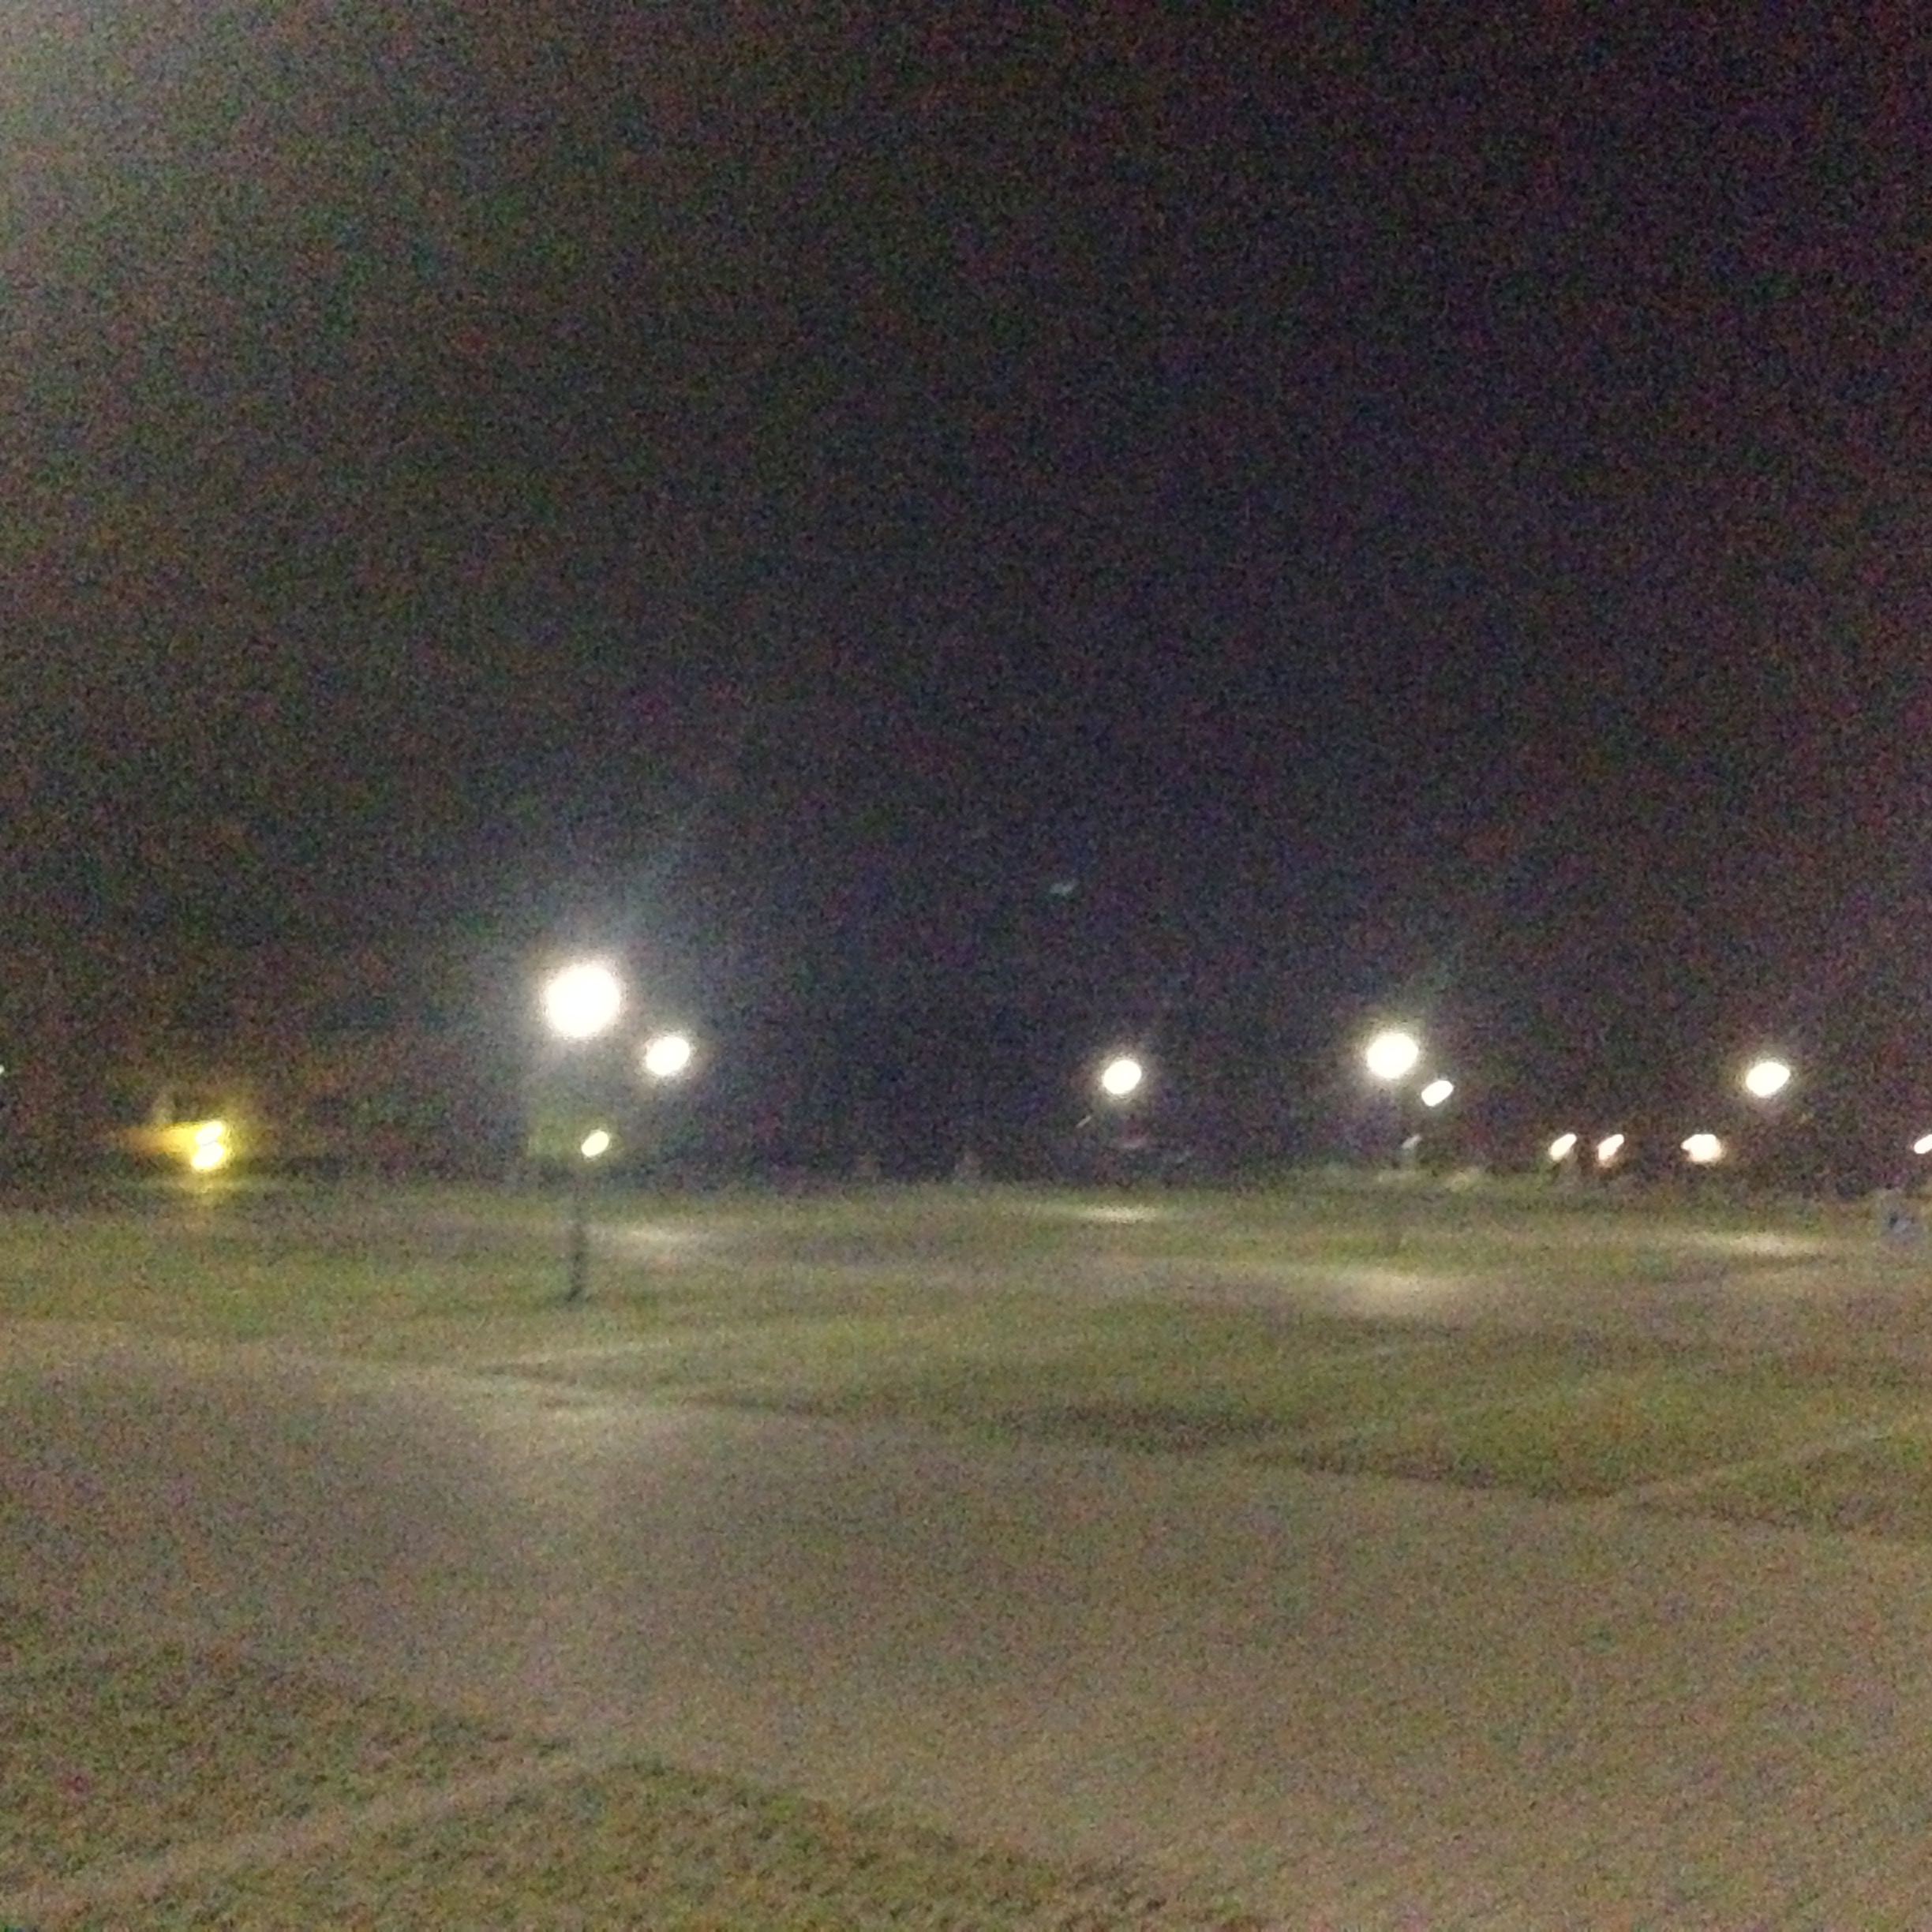
\includegraphics[width=0.2\textwidth]{Pplads.jpg}
%\caption{Illustration of the First and Second Fresnel zone, along with the Direct signal travelling from the Transmitter TX to the Receiver RX}
%\label{dijdk}
%\end{figure}


\begin{figure}
\centering
\begin{minipage}{.2\textwidth}
  \centering
  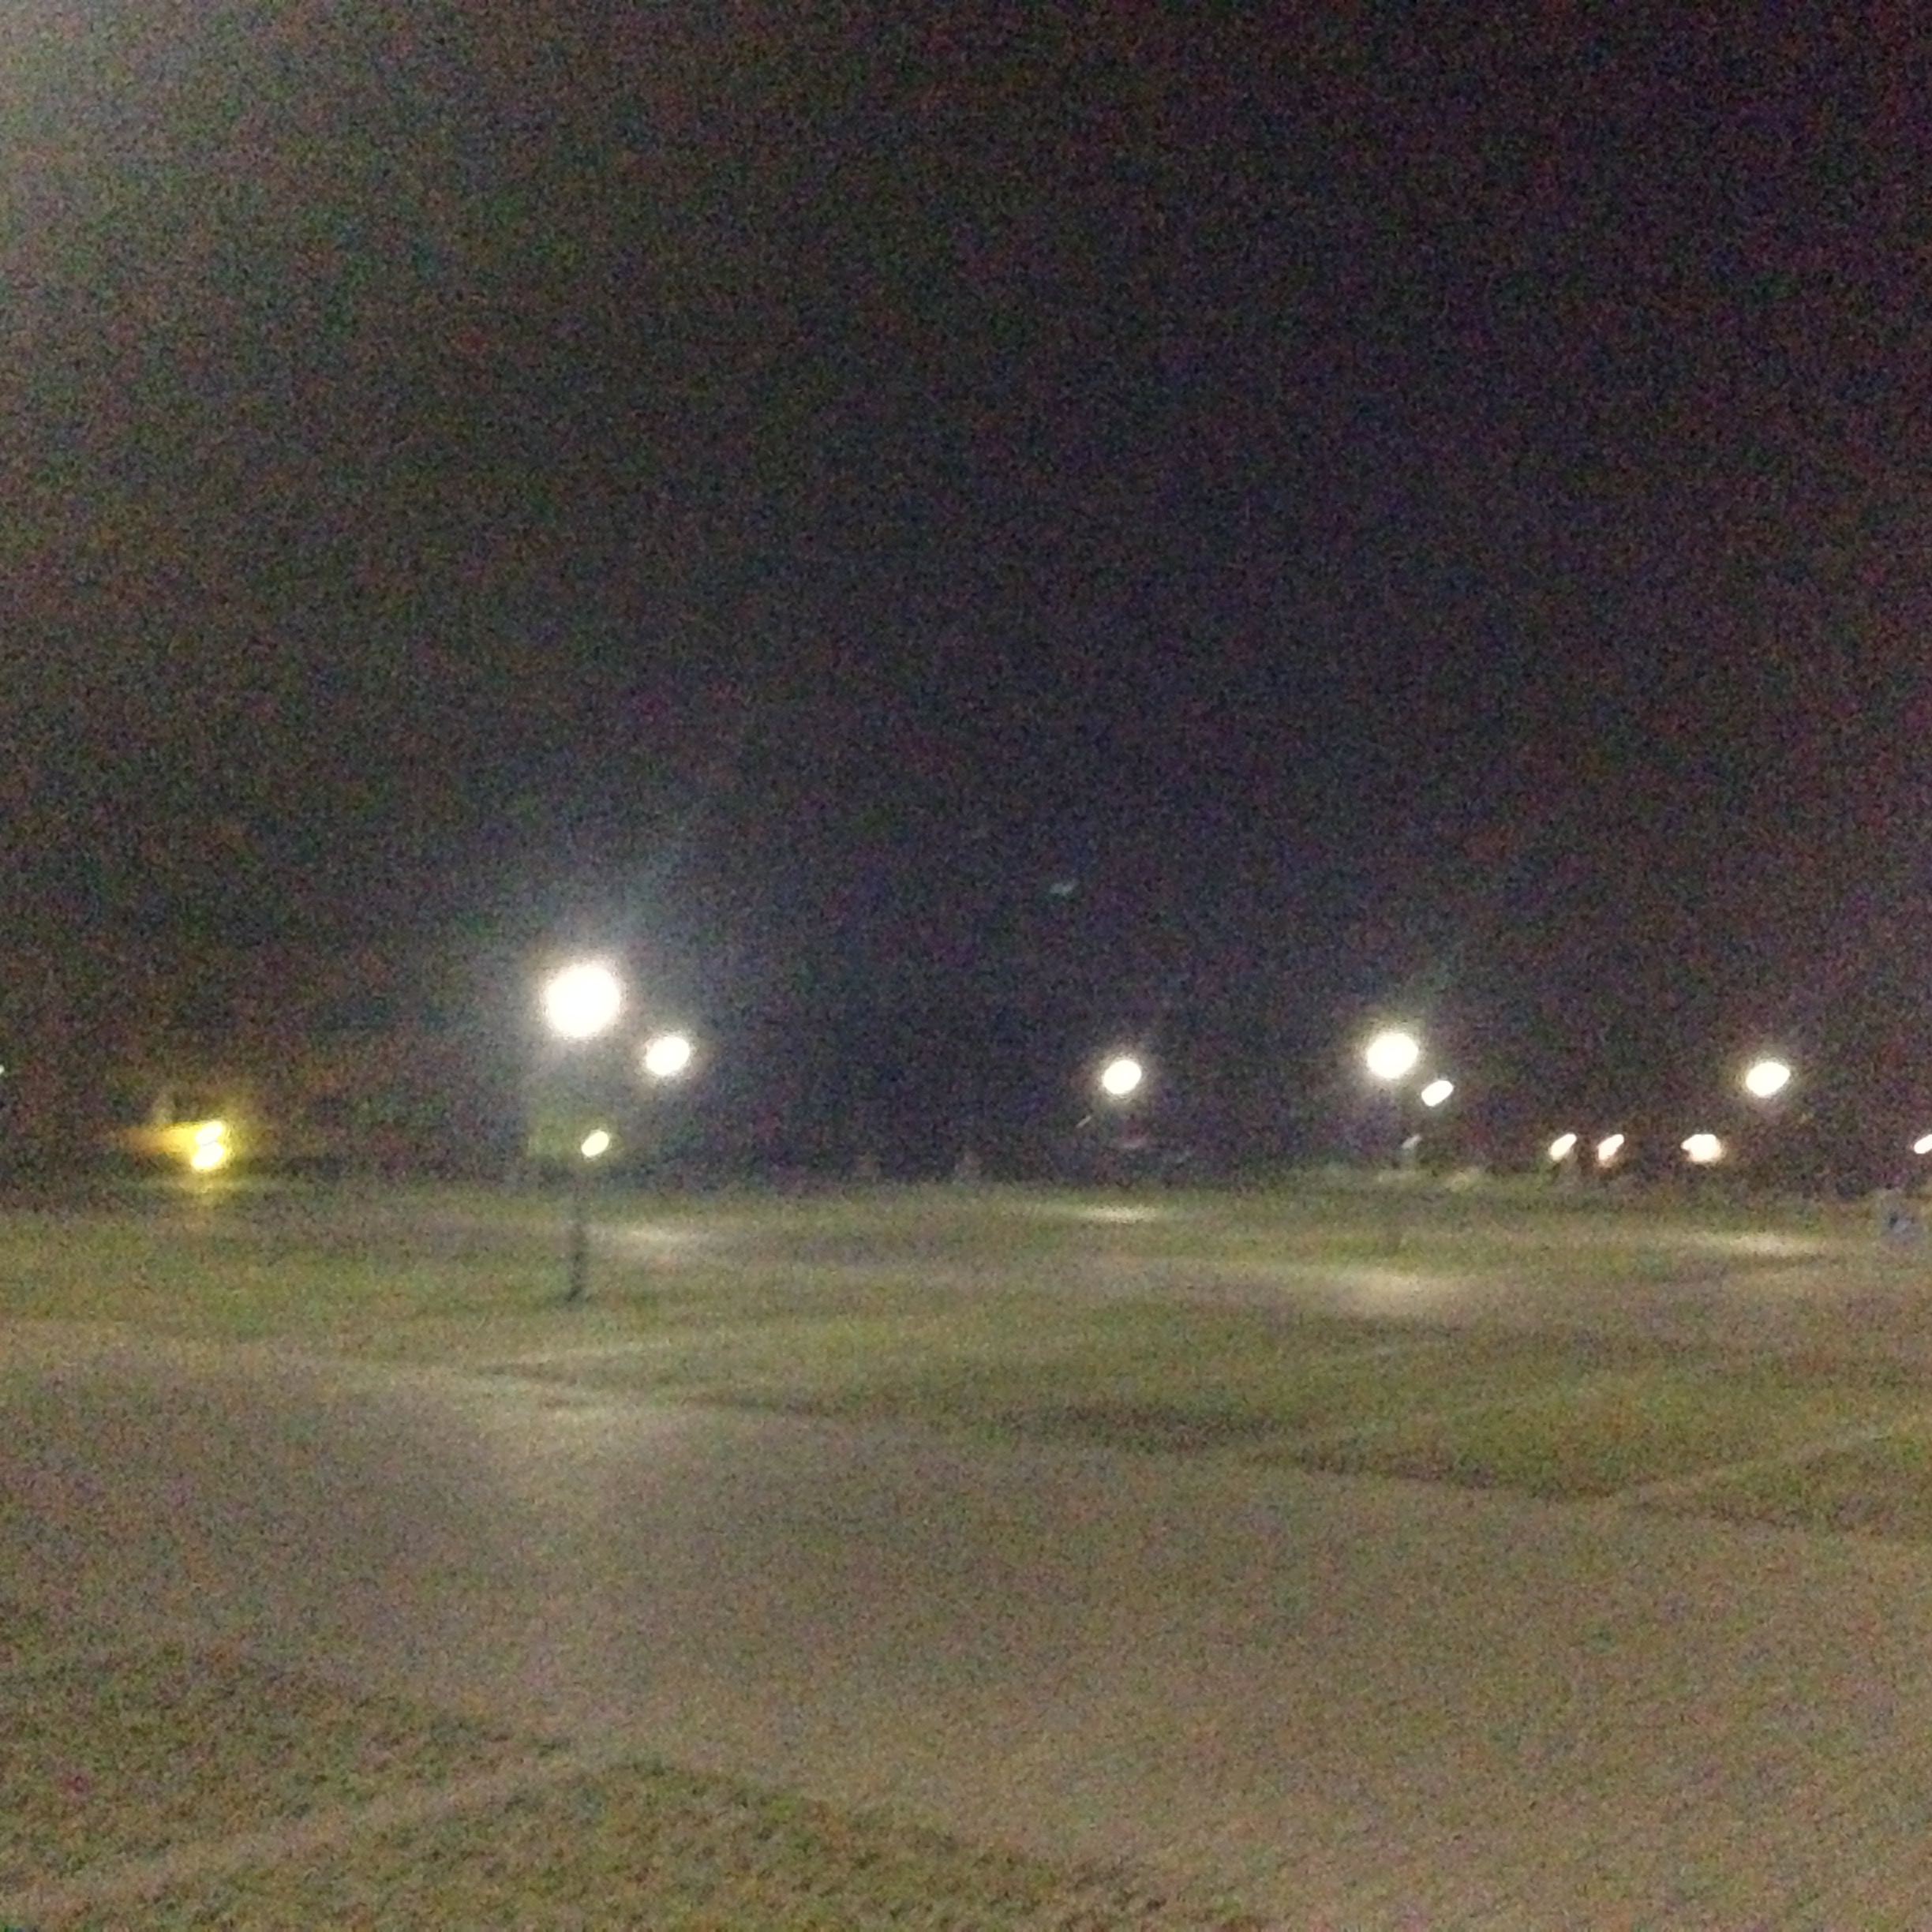
\includegraphics[width=\linewidth]{Pplads.jpg}
  \captionof{figure}{Measurement at the empty parking lot}
  \label{fig:test1}
\end{minipage}%
\hspace{2mm}
\begin{minipage}{.2\textwidth}
  \centering
  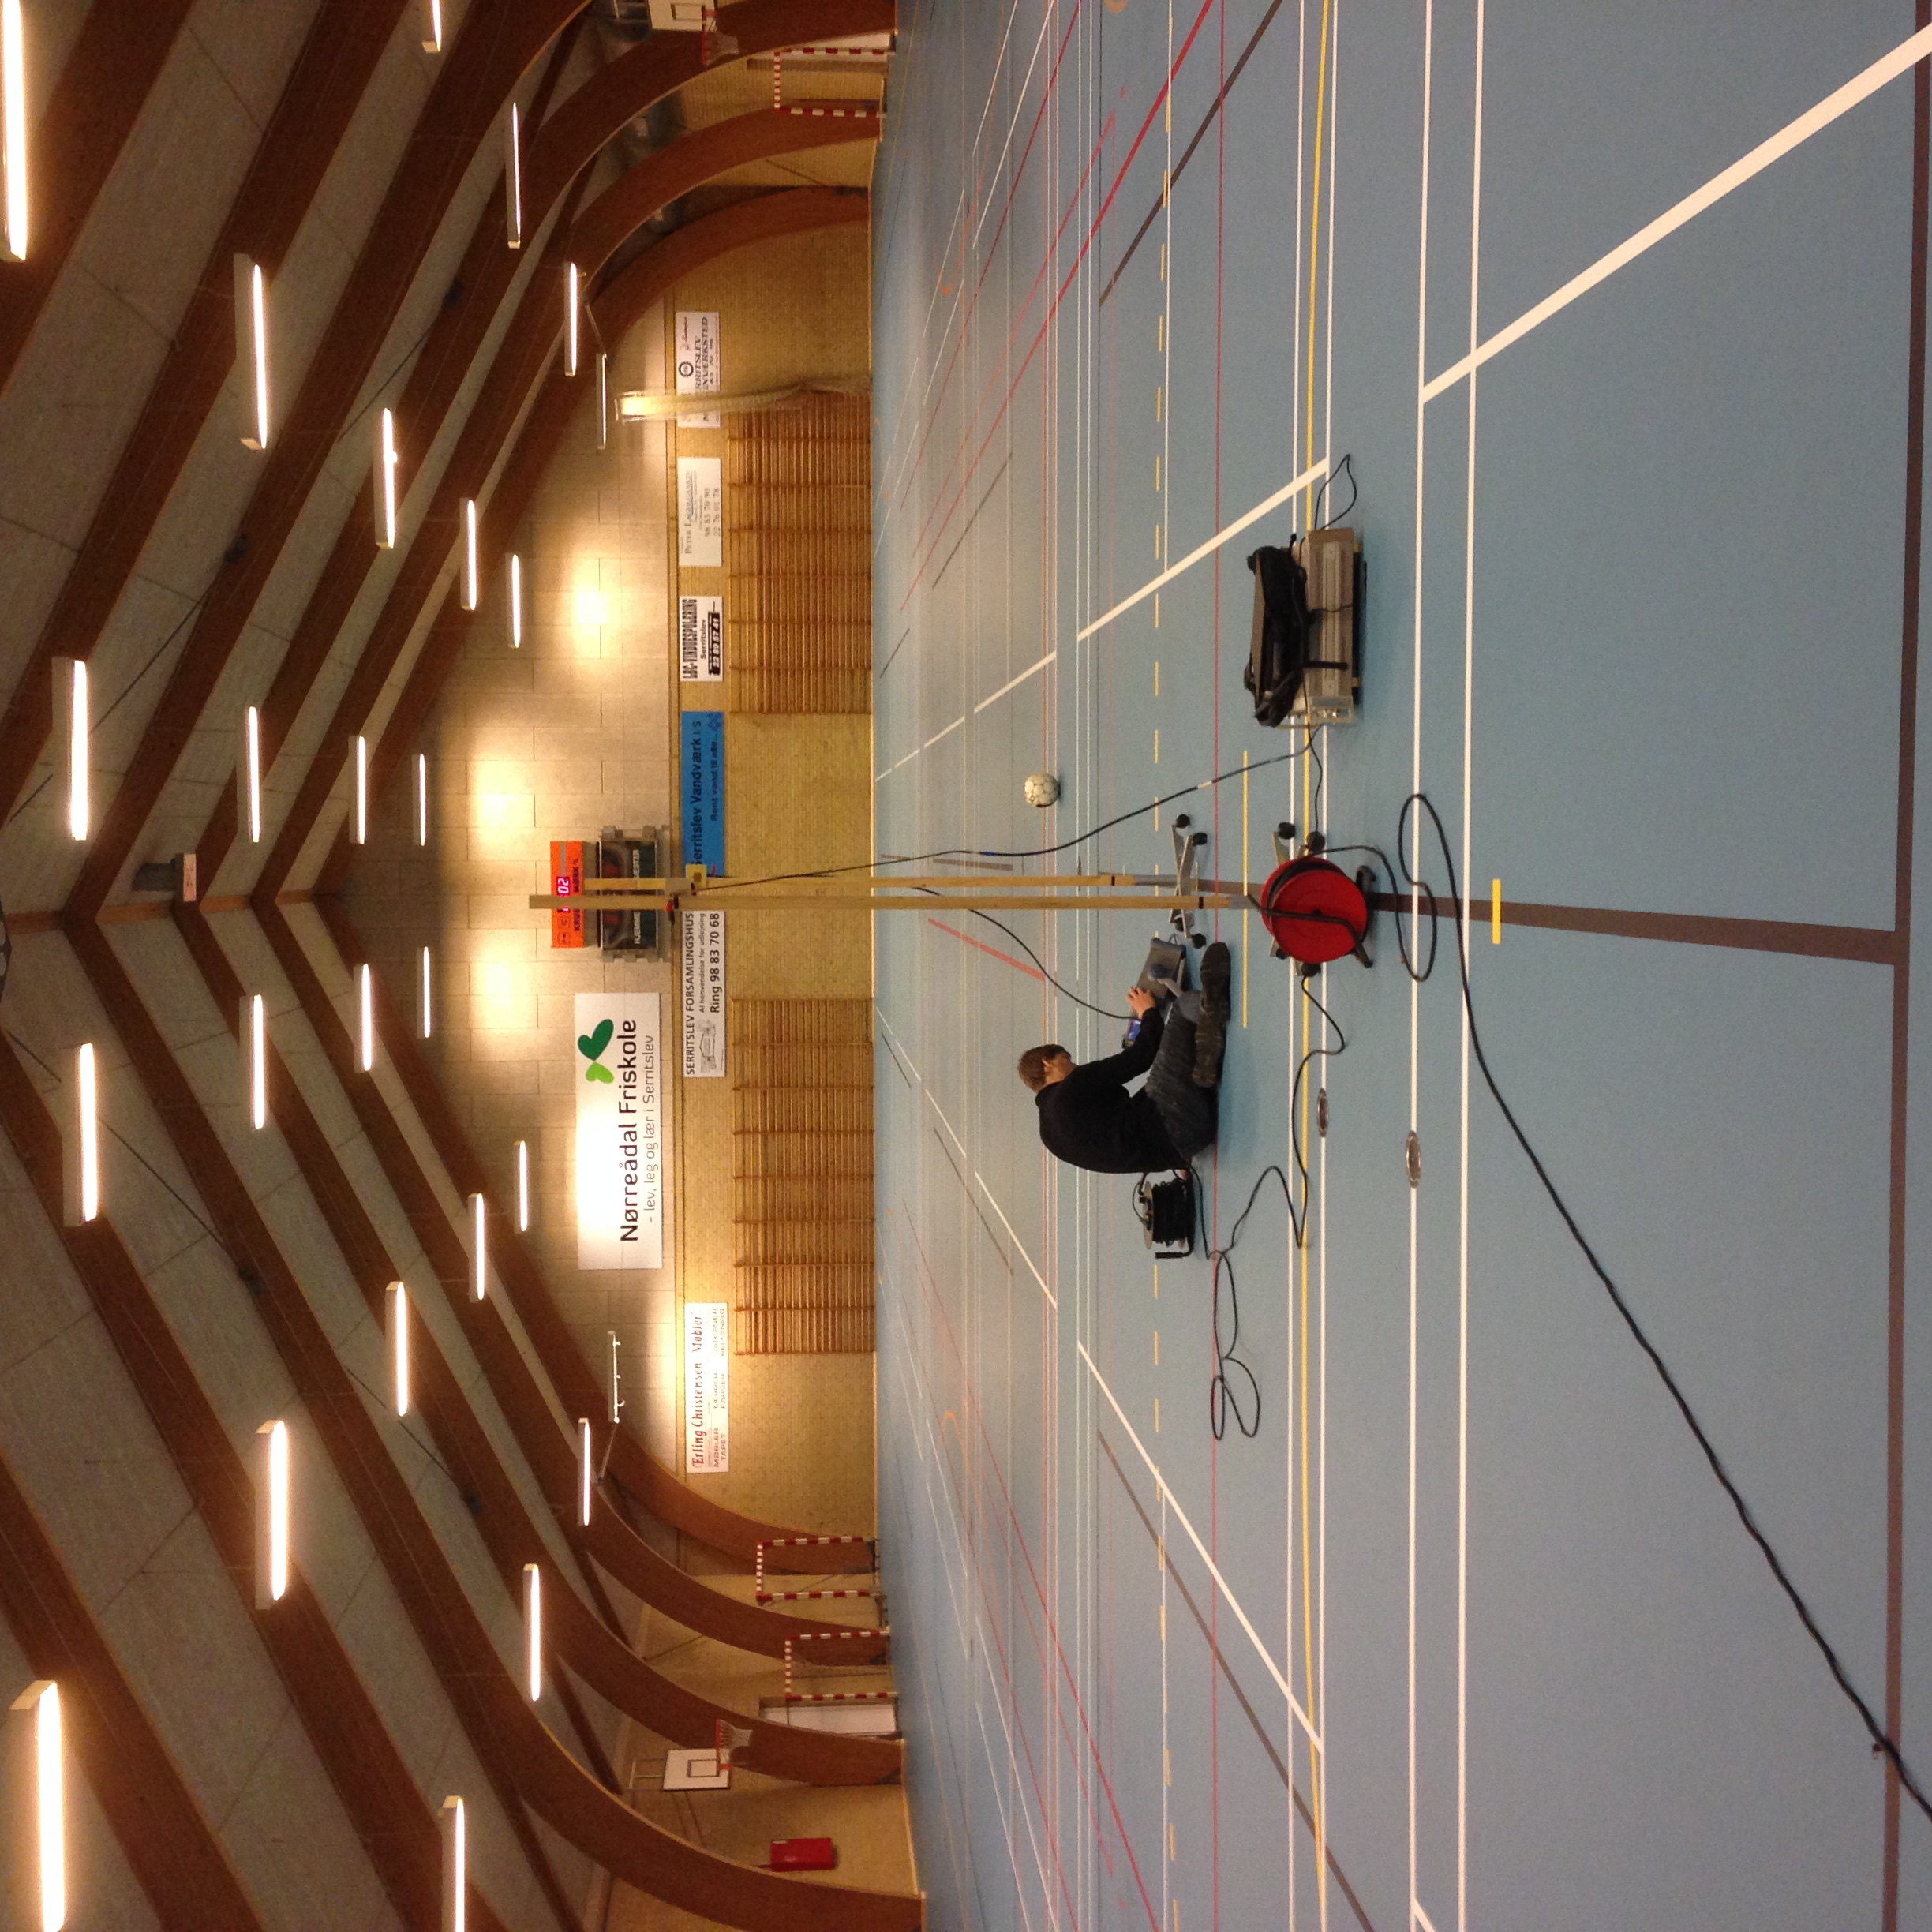
\includegraphics[angle=-90, width=\linewidth]{Hal.jpg}
  \captionof{figure}{Measurement at the gym}
  \label{fig:test2}
\end{minipage}
\end{figure}



\subsection{Subsection Heading Here}
%\input{filer/Discussion}

\subsubsection{Subsubsection Heading Here}
Subsubsection text here.

\section{Discussion}
\input{filer/Discussion}

% An example of a floating figure using the graphicx package.
% Note that \label must occur AFTER (or within) \caption.
% For figures, \caption should occur after the \includegraphics.
% Note that IEEEtran v1.7 and later has special internal code that
% is designed to preserve the operation of \label within \caption
% even when the captionsoff option is in effect. However, because
% of issues like this, it may be the safest practice to put all your
% \label just after \caption rather than within \caption{}.
%
% Reminder: the "draftcls" or "draftclsnofoot", not "draft", class
% option should be used if it is desired that the figures are to be
% displayed while in draft mode.
%
%\begin{figure}[!t]
%\centering
%\includegraphics[width=2.5in]{myfigure}
% where an .eps filename suffix will be assumed under latex, 
% and a .pdf suffix will be assumed for pdflatex; or what has been declared
% via \DeclareGraphicsExtensions.
%\caption{Simulation results for the network.}
%\label{fig_sim}
%\end{figure}

% Note that the IEEE typically puts floats only at the top, even when this
% results in a large percentage of a column being occupied by floats.


% An example of a double column floating figure using two subfigures.
% (The subfig.sty package must be loaded for this to work.)
% The subfigure \label commands are set within each subfloat command,
% and the \label for the overall figure must come after \caption.
% \hfil is used as a separator to get equal spacing.
% Watch out that the combined width of all the subfigures on a 
% line do not exceed the text width or a line break will occur.
%
%\begin{figure*}[!t]
%\centering
%\subfloat[Case I]{\includegraphics[width=2.5in]{box}%
%\label{fig_first_case}}
%\hfil
%\subfloat[Case II]{\includegraphics[width=2.5in]{box}%
%\label{fig_second_case}}
%\caption{Simulation results for the network.}
%\label{fig_sim}
%\end{figure*}
%
% Note that often IEEE papers with subfigures do not employ subfigure
% captions (using the optional argument to \subfloat[]), but instead will
% reference/describe all of them (a), (b), etc., within the main caption.
% Be aware that for subfig.sty to generate the (a), (b), etc., subfigure
% labels, the optional argument to \subfloat must be present. If a
% subcaption is not desired, just leave its contents blank,
% e.g., \subfloat[].


% An example of a floating table. Note that, for IEEE style tables, the
% \caption command should come BEFORE the table and, given that table
% captions serve much like titles, are usually capitalized except for words
% such as a, an, and, as, at, but, by, for, in, nor, of, on, or, the, to
% and up, which are usually not capitalized unless they are the first or
% last word of the caption. Table text will default to \footnotesize as
% the IEEE normally uses this smaller font for tables.
% The \label must come after \caption as always.
%
%\begin{table}[!t]
%% increase table row spacing, adjust to taste
%\renewcommand{\arraystretch}{1.3}
% if using array.sty, it might be a good idea to tweak the value of
% \extrarowheight as needed to properly center the text within the cells
%\caption{An Example of a Table}
%\label{table_example}
%\centering
%% Some packages, such as MDW tools, offer better commands for making tables
%% than the plain LaTeX2e tabular which is used here.
%\begin{tabular}{|c||c|}
%\hline
%One & Two\\
%\hline
%Three & Four\\
%\hline
%\end{tabular}
%\end{table}


% Note that the IEEE does not put floats in the very first column
% - or typically anywhere on the first page for that matter. Also,
% in-text middle ("here") positioning is typically not used, but it
% is allowed and encouraged for Computer Society conferences (but
% not Computer Society journals). Most IEEE journals/conferences use
% top floats exclusively. 
% Note that, LaTeX2e, unlike IEEE journals/conferences, places
% footnotes above bottom floats. This can be corrected via the
% \fnbelowfloat command of the stfloats package.




\section{Conclusion}
The conclusion goes here \cite{SDRPros}.




% conference papers do not normally have an appendix


% use section* for acknowledgment
\section*{Acknowledgment}


The authors would like to thank...





% trigger a \newpage just before the given reference
% number - used to balance the columns on the last page
% adjust value as needed - may need to be readjusted if
% the document is modified later
%\IEEEtriggeratref{8}
% The "triggered" command can be changed if desired:
%\IEEEtriggercmd{\enlargethispage{-5in}}

% references section

% can use a bibliography generated by BibTeX as a .bbl file
% BibTeX documentation can be easily obtained at:
% http://mirror.ctan.org/biblio/bibtex/contrib/doc/
% The IEEEtran BibTeX style support page is at:
% http://www.michaelshell.org/tex/ieeetran/bibtex/
%\bibliographystyle{IEEEtran}
% argument is your BibTeX string definitions and bibliography database(s)
%\bibliography{IEEEabrv,../bib/paper}
%
% <OR> manually copy in the resultant .bbl file
% set second argument of \begin to the number of references
% (used to reserve space for the reference number labels box)

\section*{Appendix}
To make a simplify model, there will be looked at the different test parameters, to see if some of these parameters have significant less influence on the path loss than others of the test parameters.

In the other models, the distance between the antennas and the height of the transmitting and receiving antenna is used in most of them. These parameters also influence the PL significantly. When changing the distance from from measurement point to the next measurement point, there is a rise in PL on 6 dB across all measurement.

\begin{tabular}{|c|c|c|c|c|c|}
\hline
   & 1 - 2m & 2 - 4m & 4 - 8m & 8 - 15m & 15 - 30m \\
\hline
PL & -6.54 & -7.36 & -8.44 & -8.79 & -6.12 \\
\hline
\end{tabular}

The height of the antennas influence the PL by a higher loss near ground. Shown i

\begin{tabular}{|c|c|c|c|c|}
\hline
Tx Rx & 0.01m & 0.08m & 0.34m & 2.00m \\
\hline
0.01m & -63.71 & -60.70 & -55.37 & -52.37\\
\hline
0.08m & -60.70 & -58.11 & -53.35 & -50,20\\
\hline
0.34m & -55.37 & -53.35 & -48.99 & -47.64\\
\hline
2.00m & -52.37 & -50.20 & -47.64 & -44.41\\
\hline
\end{tabular}

Compared to these two parameters, the rest of the test parameters (Placement, Antenna type and Polarization) do have a less impact, as all three parameters only have two different setups and the differences between these setups is 2.23, -4.18, 3.32 dB respectively, and there is no significantly tendencies found in the data for these parameters. This is expected for the placement and antenna type parameters, as the antenna type should not effect the PL, and the differences for the placements is found in the reflection, which have been taking into consideration for each placement. The polarization is also taking into consideration with the reflection and the antenna gains.

So for the test parameters, there will only be seen at the distance between and height of antennas. The other parameters is much smaller in influence and taking into account in other ways, so will not be looked at.



\bibliography{setup/mybib}


%\begin{thebibliography}{1}
%
%\bibitem{IEEEhowto:kopka}
%H.~Kopka and P.~W. Daly, \emph{A Guide to \LaTeX}, 3rd~ed.\hskip 1em plus
%  0.5em minus 0.4em\relax Harlow, England: Addison-Wesley, 1999.
%
%\end{thebibliography}




% that's all folks
\end{document}


